\documentclass[pdftex,12pt,a4paper]{report}

% Document settings

\usepackage{fullpage}
\usepackage{cite}
\usepackage{datetime} 
\usepackage{geometry}
\usepackage[pdftex]{graphicx}
\usepackage{verbatim}
\usepackage{todonotes}
\usepackage{array}
\usepackage{capt-of}
\usepackage[parfill]{parskip}
\usepackage{underscore}
\usepackage{url}
\usepackage{listings}
\usepackage{fancyvrb}


 \usepackage{courier}
 \lstset{
         basicstyle=\footnotesize\ttfamily, 
         numberstyle=\tiny,      
	language=Java,
 }
 \lstloadlanguages{
         Java
 }

\makeatletter
\g@addto@macro\@verbatim\small
\makeatother

\geometry{verbose,lmargin=3cm,rmargin=3cm}

\newcommand{\HRule}{\rule{\linewidth}{0.5mm}}

\begin{document}

\begin{titlepage}
\begin{center}

% Upper part of the page. The '~' is needed because \\
% only works if a paragraph has started.

\includegraphics[width=0.4\textwidth]{figure/crest.png}~\\[1cm]

\textsc{\LARGE Imperial College London}\\[1.5cm]

\textsc{\Large Final year project}\\[0.5cm]

% Title
\HRule \\[0.4cm]
{ \huge \bfseries Computer Music Improvisation \\
A Grammatical Approach For Jazz}\\[0.4cm]

\HRule \\[1.5cm]

% Author and supervisor
\begin{minipage}{0.4\textwidth}
\begin{flushleft} \large
\emph{Author:}\\
Cliff \textsc{Sun} \\
chs09@ic.ac.uk
\end{flushleft}
\end{minipage}
\begin{minipage}{0.4\textwidth}
\begin{flushright} \large
\emph{Supervisor:} \\
Professor Murray 
\textsc{Shanahan}
\end{flushright}
\end{minipage}

\vfill

% Bottom of the page
{\large \today}

\end{center}
\end{titlepage}

\chapter*{Abstract}%
\addcontentsline{toc}{chapter}{\numberline{}Abstract}%
...
\chapter*{Acknowledgements}%
\addcontentsline{toc}{chapter}{\numberline{}Acknowledgements}%
...


\setcounter{tocdepth}{2} % Set the depth of toc indexing

\tableofcontents

\pagebreak

\renewcommand*\thesection{\arabic{section}}
 
\pagebreak

\chapter{Introduction}

\section{Overview}
Improvisation is often seen as a human activity, especially in the domain of music. Genre's such as Jazz and Blues are heavily based on the performer improvising on a set form. Improvisation is also seen as an activity that involves creative processes and as such improvisation is seen as a creative process itself. In addition a large part to being able to improvise jazz is the large set of skills and rules with accompanying music theory that needs to be learnt by the performer. In this regard, we can say that jazz as a genre lends itself well to a project based on computation creativity. However it is difficult to tell how much of the creative aspect of improvisation is based on the rules and music theory behind jazz, or even what aspects of the music produced is down to creativity. Thus capturing the creative processes behind improvisation is much harder to describe. The aim of this project is to be able to model and replicate such music improvisation using a computer. There have been many different approaches for melody generation/improvisation in blues and jazz over the years and many of them have involved a statistical/machine learning approach. We explore a more grammatical approach which uses an abstract musical grammar which will allow us to create well-defined structures and rhythms for jazz melodies. The area of computational creativity in music has been explored before and is still ongoing, and we hope that this project can provides a different insight for computer music improvisation. 

\paragraph{Improvisation vs Composition}
Music improvisation can be defined as the creative activity of immediate composition, or 'Composition on the fly'. In the case of this project, both terms will be used interchangeably. However, the act of improvisation usually encompasses the playing itself, whereas composition can be seen as just composing notes for playing later. Our project is not designed to solve the playing aspect of improvisation, and is better stated that our project essentially composes jazz solo's in the style of jazz improvisation.

\section{Motivation \& Aims}
Many current and past approaches use analytical methods (i.e. mathematical and statistical methods), i.e. they try to capture and abstractly learn the creative process of improvisation from jazz pieces/examples. I.e. they start from the end and they try to learn and infer the rules and constraints for improvising in the same style as the example. In addition, many approaches also treat the pitch and the duration of a note as coupled objects. 
However what if we were to describe the rules and constraints ourselves? Just like any activity, Jazz improvisation is governed by many 'rules' (though it is important to recognise that they don't necessarily need to be followed all the time). In the case of actual notes/pitches, musical theory (specific and non specific to jazz) plays an important role for improvisation, telling us which notes we could use in a certain section in the piece (which scales are feasible with which chords). Musical theory is extremely complex especially when dealing with scales and harmonies (as we shall see later in Chapter 2). One of our aims is to be able to capture as much of the comprehensive set of musical 'rules' as we can into a knowledge base for the program. Therefore one of the questions that we are trying to answer is that how does having a extensive knowledge base itself affect the quality of the output? Additionally, on the subject of rhythmic ideas in jazz, one of the constraints that we explore in this project is the use of an abstract grammar to produce abstract tone sequences. Such an abstract grammar constraints the rhythmic sequence of our notes whilst also constraining the type of notes that we can use. We aim to produce a general solution which can take in a grammar specified by the user to generate jazz music with, thereby not limiting the possibilities of what can be generated. This forms the main body of the project and will be explored into detail in Chapter 4.

\section{Project Domain - Computational Creativity}
The project comes under the area of computational creativity, and it's immediate uses and contributions are fairly novel. We could say that one of the main challenges of computational creativity is to encapsulate the creative processes of a human being into a computer. This is a non-trivial task as such, the human brain is an extremely complicated entity with which we still do not have a full understanding of and thus it is difficult to define what creativity objectively means. On the other hand, computational creativity can also help us understand further the behaviour of creativity in humans. As a result, a project in the field of computational creativity is often very experimental in terms of its approach and it's end result. 

Much work has been done in the field of generated visual art with tools and programs such as Simon Colton's Painting Fool \cite{website:paintingfool} and Harold Cohen's AARON \cite{website:aaron} both of which create original artistic images to a high standard.

Evaluation of such projects is not easy, usually such projects will produce an output of an artistic form (music/art/literature) and as such evaluation can be very subjective depending on the person. A simple way we can evaluate the output and result of such a project (in terms of music) would be to do a blind test to compare a similar human composed piece of music to the output of the new program. We can score the program and its output based on whether the listener can or can not identify which piece of music was compose by a computer and which was composed by a human and which they preferred. In addition we will also use Simon Colton's FACE descriptive model \cite{coltonface2011} This will be explained more in the Evaluation section.

\section{Related Works}
Work on computer music improvisation dates back 20-30 years or so. One famous example of computer generated music in general is David Cope's EMI (Experiments in Music Intelligence) which produces music in the style of various composers (using existing works as input sources). In terms of computer improvisation for jazz and blues music, there have been numerous analytical (statistical and mathematical) approaches. One such approach based on machine learning techniques includes 'Finding temporal structure in music: Blues improvisation with LSTM recurrent networks' By Eck and Schmidhuber (2002) \cite{eck02}. Belinda Thom's Band-out-of-a-Box (BoB) describes an interactive soloist which can improvise with another performer using unsupervised learning in 'Unsupervised Learning and Interactive Jazz/Blues Improvisation' (2000) \cite{thom2000}. In addition Markov chains have been used to analyse and model jazz improvisation such as 'Markov Chains as Tools for Jazz Improvisation Analysis' by Franz (1998) \cite{franz98} and 'Improvising Jazz With Markov Chains' by Marom (1997) \cite{marom97}.

Other works regarding grammatical approaches for music improvisation include approaches based on string rewriting grammars (L-systems) in 'Grammar Based Music Composition' by McCormack (1996) \cite{mccormack96}. In addition 'A Grammatical Approach to Automatic Improvisation' by Keller and Madison \cite{keller07} introduces a formal grammar for music improvisation in which we will be basing our work on (see more below).

In addition and in relation to Keller's above mentioned paper \cite{keller07} we also note that work has also been done by Keller to learn jazz grammars from a corpus of jazz melodies. Learning Jazz Grammars by Gillick, Tang and Keller \cite{kellergillick09} uses a machine learning approach (combining clustering and markov chains) to learn abstract grammars which can be used to produce jazz melodies (similar to the system that \cite{keller07} produced). 


\section{Report Outline}
The rest of the report is laid out as follows:
\begin{description}
  \item[Chapter 2] provides some background on music theory and in particular some Jazz theory and ideas that are commonly used to improvise Jazz with.
  \item[Chapter 3] describes a simple approach without using a grammar to allow us to contrast the differences between grammatical and non-grammatical approaches
  \item[Chapter 4] describes the main grammatical approach that we have used, based on Keller's paper \cite{keller07}. We also provide background on context free grammars and also describe the heuristics we have used to generate the actual musical notes.
  \item[Chapter 5] describes a novel extension which allows the program to update the input grammar weightings using the user/listener as a fitness function / the evaluator.
  \item[Chapter 7] explains the evaluation process that we have gone through to measure the success and achievement of the project. This includes surveying users on comparing human composed jazz and computer composed jazz (from this project) and in addition we use some models/criteria for measuring the 'creativeness' of our final program.
\end{description}

\pagebreak

\chapter{Background - Musical Theory}

\section{Overview}
In this chapter we aim to provide some background on musical theory that is used in jazz and musical theory overall. We assume that the reader has some basic music theory knowledge on scales and chords already


\section{Blues Improvisation}
Blues is one of the most common genres that relies on performer improvisation. Performers of this genre tend to play a musical instrument (including voice) on top of an accompaniment with a well defined structure/form. The blues form itself is often defined by its 12 bar chord progression (commonly called 12 bar blues) which is essentially a standard harmonic chord progression of 12 bars in a standard 4/4 time signature. Table 1.1 below shows the chords for the general 12 bar blues form, with I7 referring to the harmonic seventh Tonic chord. Chord IV refers to the 'dominant' chord (4th degree) and Chord V refers to the 'dominant' chord (4th degree).

\begin{table}[here]
\centering
\newcolumntype{C}{>{\centering\arraybackslash}m{23pt}<{}}
\begin{tabular}{|*{12}{C|}}
  I & I or IV & I & I7 & IV & IV & I & I7 & V & V or IV & I & I or V
\end{tabular}
\caption{12 bar blues chord progressions}
\label{12 bar blues}
\end{table}


\begin{table}[here]
\centering
\newcolumntype{C}{>{\centering\arraybackslash}m{23pt}<{}}
\begin{tabular}{|*{12}{C|}}
  I & I & I & I & IV & IV & I & I & V & IV & I & I
\end{tabular}
\caption{12 bar blues simplified chord progression}
\label{12 bar blues}
\end{table}

Table 1.2 gives us one possible (and simple) chord progression for 12 bar blues in which we will basing our improvisation upon. 

\subsection{Blue Notes} What really gives the blues genre it's characteristics are the 'blue notes'. These are notes which are played at a lower pitch (flatter) than that of the major scale (usually one semitone lower on piano). The notes which are 'flattened' are the \textbf{third}, \textbf{fifth} and \textbf{seventh} notes of the major scale.
There are theoretical reasons for the introduction of 'blue notes' which we won't go into detail here. But essentially these 'blue notes' allow for moments of expression in blues melodies. 

\subsection{Blues and Pentatonic Scales}
Blues scales include the blue notes that we've mentioned above, these scales give the performer a set of notes to improvise with and gives the music the characteristic 'blues' feel to it. Blues scales are generally based on the major/minor pentatonic scale. A pentatonic scale is a scale of five notes (compared to seven notes in regular major/minor scale) and is widely used in music across the world. The most common blues scale (and the one we are going to be basing our improvisations on) is the blues minor scale which is based on the minor pentatonic scale (see Figure \ref{fig:cminorpentatonicscale}) with a sharp 4th note (or a flat 5th note, both are equivalent). In Figure \ref{fig:cminorbluesscale} we can see the blues minor scale includes all the blue notes; E(3rd degree) flat, G(5th degree) flat and B(7th degree) flat.

\begin{figure}[here]
  \centering
  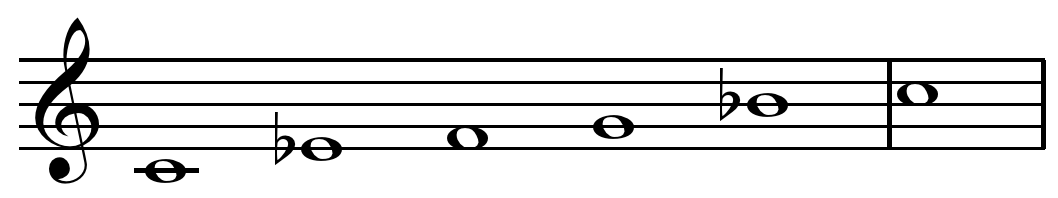
\includegraphics[scale=0.25]{figure/minorpentatonicscale.png}
  \captionof{figure}{C minor pentatonic scale}
  \label{fig:cminorpentatonicscale}
\end{figure}

\begin{figure}[here]
  \centering
  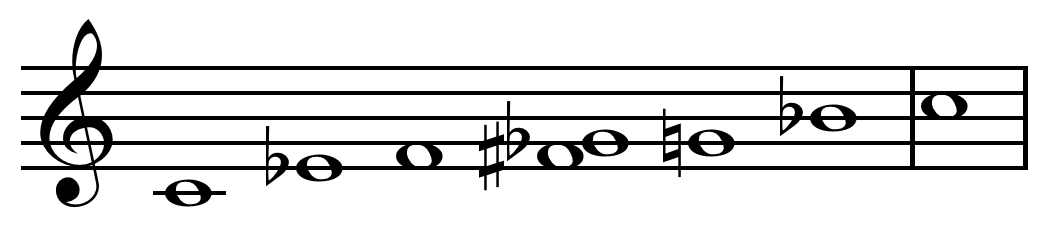
\includegraphics[scale=0.25]{figure/bluesminorhexatonicscale.png}
  \captionof{figure}{C minor blues (hexatonic) scale}
  \label{fig:cminorbluesscale}
\end{figure}

\section{Jazz Improvisation}

\subsection{Versus Blues}
Though it is common to use terms blues and jazz interchangeably, the reality is that they are very much different styles of music. However it is very difficult to categorise these two genres of music and much of the genre is overlapping. We'll refer to our music as fitting both jazz and blues during this report.

Blues itself has a very simplistic style, it relies on basic chord progressions (I IV V as we've seen above) which are repeated over and over again. By using one scale (pentatonic or minor blues scale) we can easily improvise a melody on top of the progression. In addition feeling and emotion is important in blues music and thus blues is based more on expression rather than technical ability. 

Jazz has many roots in blues music (in fact the blues form is ubiquitous in jazz music), the 12 bar progression is commonly used in Jazz music in addition to blue notes for expressive purposes. However Jazz itself is much more complex than blues and uses many more chords/scales, time signatures and melodic structures than blues. For example Jazz's rhythms tend to use syncopation (playing on the off beat) and swung notes i.e. playing two notes (which have the same duration) with different durations, where the first note has the longer duration and the second one the shorter. In addition Jazz chord theory itself is a very complicated as we shall see below.

\section{Basic Jazz Theory}
Jazz theory is extremely comprehensive and reflects in the complexity and the range of the music that belongs to this genre. It is useful to explain some musical theory that will not only help us understand improvisation, but music composition in general. Note that there is no right or wrong way to play music, there are many oddities in how the harmonic aspect of music works. Music theory (emphasis on the 'theory') itself only aims to formalise (and standardise) a set of rules for music knowledge. In terms of jazz theory, books such as 'The Jazz Piano Book' by Mark Levine provide a comprehensive learning guide to aid and teach jazz pianists the complex chord theory that jazz imposes. As it covers almost everything a beginner/intermediate jazz pianist needs to know to be able to improvise/play jazz, we will not go through everything from the book here. But we will highlight some of the more relevant ideas that we are using in our project.

\subsection{Chord Voicings}
Often a good way to start/learn simple jazz improvisation is to learn jazz chord voicings, these are essentially accompanying chords in the left hand which allows the pianist to use their right hand to play the melody and improvise. Chord extensions can be used to provide variations in the left hand voicings, for example adding the sixth, ninth and thirteenth scale note to the chord. Various progressions can be constructed using the large vocabulary of chord voicings, though many are based on the same underlying basic progression.

\subsection{Chord Substitution}
Chord substitutions are very common in Jazz, where a player/composer would use a chord in place of another related chord. Often it is just changing a note or two in the chord, but this small change often creates variety and interest and is what gives jazz music it's harmonic and melodic variety. The theory behind this is fairly complex and we won't be exploring this further, but the idea is that chord substitutions are possible and allow a richer variety in the music.

\subsection{Scale Theory - Playing Off the Chord}
As explained previously chord voicings allow us to have a varied left hand accompaniment which allows the right hand to improvise melodies. One simple way we can improvise melodies is to use scales that fit with the chord voicings. Indeed much of jazz is based on playing over the chords and being able to follow the chord changes itself. Certain scales fit different chords and thus it is up to the performer to choose the right scale to use to improvise a melody. Note that when we talk about scales here we do not mean in terms of sequence of notes, but rather the collection of notes that belong to the scale.

\subsubsection{Scales \& Modes}
For a simplified example, we can say that in the key of C major, the C major scale can be used over the II, V and I chord, i.e. Dm(7), G(7) and C. This is because for each chord, the 3rd and 7th note exists in the C major scale. We've discussed previously that the 3rd and 7th of a chord and scale indicates/identifies the tonality of the chord and scale. Thus it is reasonable to point out that scales with the same 3rd and 7th as a chord can be used to improvise on top of the chord.
If we look at it from another approach, then we can say that the chords used (and the tonality of the chords, i.e. major/minor/dominant) for the progression can be derived directly from the C major scale itself. To do this we must introduce an important piece of musical theory called modes. A mode is essentially a scale that can start from anywhere (not just the tonic C). There are 7 different modes in C major, each mode (scale) starting from a different note in the C major scale, below is an example of the 7 modes in C major and their corresponding names  \cite{jazzmusicmakers}.

\begin{figure}[here]
  \centering
  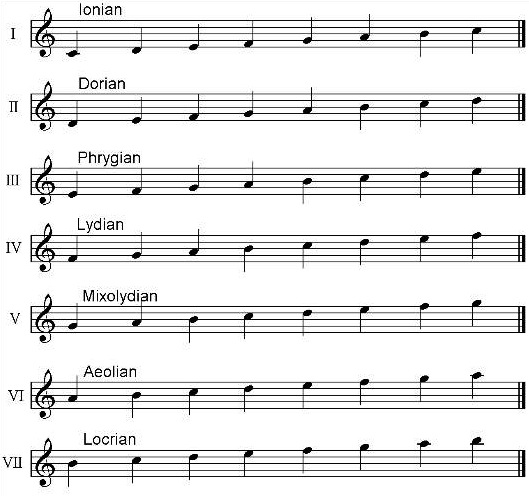
\includegraphics[scale=2.7]{figure/cmajormodes.jpg}
  \captionof{figure}{Modes for the C major scale}
  \label{fig:cmajormodes}
\end{figure}

If we look at the second (Dorian) mode we see that it starts from D and has an F natural and a C natural (3rd and 7th note respectively). This does not correspond to any D major/minor scale, which gives us the reason for having modes (allowing us to express and formalise different sequences of notes). If we take the 1st, 3rd and 7th of the Dorian mode, we get a D minor 7th chord (D, F, C), i.e. the II chord in our above progression. Similarly, if we take the fifth (Mixolydian) mode which starts from G, and we take the 1st, 3rd and 7th notes, we end up with a G dominant 7th chord (G, B, F). C major Ionian mode is trivial and thus we have our basic II-V-I progression derived from C major and it's modes. 
These modes also point out to us the avoid notes for each chord. The avoid note generally tends to be the 4th note, i.e. for the G7 chord, we use the fifth (Mixolydian) mode, where the C is the avoid note. This is because if you were to play a C on top of the G7 chord, it would sound dissonant. But avoid notes themselves can be used as passing notes where they don't have as much of a tonal impact in the music. As such, when we are in the key of C major and we have a dominant seventh chord in our left hand (G7), we can use the Mixolydian scale to improvise on top of the G7 chord. The above theory constitutes Major scale harmonies. It is also possible to 'raise' the 4th note (augmented, annotated as +4) as an alternate to having the 'avoid' note. For example we may use the first mode in C major (Ionian) and raise the 4th (F natural) to F sharp. We can see the effect of this \ref{fig:clydian} taken from the Jazz Piano Book. In effect we have changed the key and as such the key happens to be G major. This means the new scale is in fact the C Lydian mode (in G major). However raising the 4th does not always in effect give us a new mode which corresponds to a different (major) key. Sometimes the new scale does not match any major key but rather is based on melodic minor scales. This brings us to Melodic Minor scale harmonies, however we won't go into this further, but it is important to realise the complexity of scales and scale theory not only for jazz, but for music in general.

\begin{figure}[here]
  \centering
  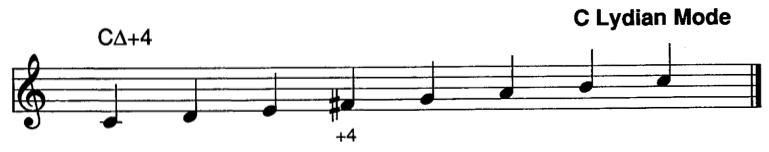
\includegraphics[scale=0.45]{figure/clydian.png}
  \captionof{figure}{C Lydian mode (in the key of G major)}
  \label{fig:clydian}
\end{figure}

Note in summary that it is important to think about the key that we are playing in, rather than the specific chord. We may end up using scales that are actually modes in alternative keys, which gives us musical variety in the improvisations.

\subsection{Chord - Scale System}
Following on from previously, the different scales and modes that we can use provide us with many alternative scales to use for improvisation over different jazz voicings. Different combinations of scales and chords have been used and developed over the years by the great jazz musicians, many of which had their own preferences for which types of scales to use for which voicings. This gives us a very diverse sound in jazz music and is what gives different players and musicians their own distinct style. 

\subsubsection{Dissonance - Avoid Notes} \label{avoidnotes}
One of the main concerns with the chord scale system is how it handles dissonance. Dissonance occurs when you have a combination of notes that sound harsh and unpleasant to the listener. In jazz music when using certain scales with chords, we may have some notes that we should 'avoid' as they sound harsh when played with the chord. Therefore they are known as 'avoid' notes. However in reality we can use avoid notes as passing notes, i.e. notes that will resolve to a more harmonic note. [example]

\begin{figure}[here]
  \centering
  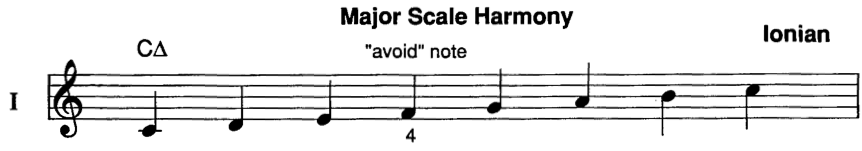
\includegraphics[scale=0.4]{figure/cionian.png}
  \captionof{figure}{C Ionian mode (in the key of C major)}
  \label{fig:cionian}
\end{figure}

Here we see that for a c ionian scale, with its accompanying chord, c major 7th chord ($\Delta$ indicates a major 7th chord), the F (the 4th/11th note) would be the avoid note.  In general for a major seventh chord (as we see above), the 4th note in the accompanying major scale is always the avoid note. But this is not necessarily the case for minor melodic scales, therefore it is not easy to determine which notes are 'avoid' notes. One way of defining avoid notes (which is not quite definitive in reality) is that the avoid notes tend to be the notes that are a half step (semitone) above the chord tones (1,3,5,7 intervals of the chord for example).

Overall it will be quite difficult to include all the scales and modes for major, minor and other harmonies. However our aim is to be able to represent the chord and scale theory as best as we can.

\section{Computer Improvisation For Blues/Jazz}

\subsection{Overview}
The idea behind jazz improvisation on the computer is that whilst jazz is essentially composition during performance (composition concurrent/on the fly), the composition is not completely done on the spot. Jazz musicians will practice many jazz licks, voicing's and scales before hand so that they can go into a performance with the required knowledge and practice needed to improvise jazz. Blues is also similar, blues musicians will practice pentatonic and minor blues scales whilst learning blues/jazz licks. Prior knowledge (knowledge of chord and scale theory) is a definite requirement in order be able to improvise blues/jazz at an advanced level.

\subsection{Difficulty/Complexity}
Blues and jazz music can range from something extremely simple such as playing the minor blues / pentatonic scale over a variation of the 12 bar blues progression, to complex theory involving left hand voicings, chord substitutions (tritone substitutions for example) and scale theory (and scale modes as we saw previously). Our aim is to be able to incorporate and encapsulate as much jazz theory as we can in the system that we are developing such that it can produce music with vast melodic and harmonic variations. Strictly speaking, the music that we generate may not strongly adhere to either a blues/jazz style (i.e. it may not easily identified with a jazz sub-genre or with a famous jazz musician) but is rather based on the ideas of blues and jazz improvisation. In addition the aim is to be able to provide a general solution that does not just produce a limited style and sound but rather be able to improvise a melody on any chord progression that we can give it. As a starting point, our goal is to generate/improvise jazz blues melodies on top of a 12 bar progression using a computer. Musical improvisation also covers improvisation/variations for the accompaniment as well. A grammar for comprehensive chord substitutions in improvising accompaniments in 12 bar blues/jazz is covered in Steedman's paper 'The Blues and the Abstract Truth: Music and Mental Models' \cite{steedman96}. However in this project our main focus is on melody generation.

Due to the project's time constraints and the complexity of jazz music, we are only aiming to be able to produce something that improvises jazz music to a beginner/intermediate level. The main challenge behind this project is the experimentation and uncertainty of using a grammatical approach to improvise music. Having a more realistic/achievable target (producing beginner's level jazz music) we have simplified the overall problem which allow us to concentrate on the technical aspect of the project.

\paragraph{Keys}
It is well known that the characteristic of music i.e. the listening experience is not based on the pitches of each note, but the pitch changes between each note. Thus a melody played in different keys will be recognisable to any listener familiar with the melody. For this reason we can simplify our problem further by working (melody generations/chord progressions) in the same key, the key of C. Transposition can be easily done by external tools and packages.

\pagebreak

\chapter{Initial Non-Grammatical Approach}

\section{Overview}
Before diving into a grammatical approach for blues melody improvisations, we decided to explore some simple ideas regarding probabilistic generation of notes in a sequence. Below are two simple approaches that we took. Note that we could easily classify these approaches with a simple grammar, however the point of introducing a grammar is so that we can defined structure and rhythm in our melodies, so for now we say that the first two simple approaches/implementations are not a 'grammatical' approach. 

\subsection{Simple Probabilistic Generation (with fixed duration)}
We decided to make a quick music improvisation tool which uses probabilities to pick the next note in the melody. We kept the duration constant (a quaver/eighth note) and kept the range within one octave. An example of the generation is shown below in Figure \ref{fig:randomgeneration}. We designed it so that the probability that we choose the next note has an inverse relation to the interval of the note itself. I.e. the probability is of choosing an adjacent note in the blues scale is highest, with the probability for choosing a note that is 2 notes apart lower. In addition we made it so that the probability that we choose a note so that sequence is going in the same direction is higher than choosing a note that changes the direction of the sequence. For example if we had an F (natural) followed by an F\#, the probability of choosing G is higher than choosing an F (natural) (both one note interval from F\#).

\begin{figure}[here]
  \centering
  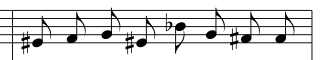
\includegraphics[scale=0.7]{figure/randomgeneration.png}
  \captionof{figure}{Probabilistic generation for a blues sequence}
  \label{fig:probabilisticgeneration}
\end{figure}

In the figure above we can see that a probabilistic random generation of notes with some constraints yields a fairly decent result. The notes are all part of the blues scale and so sound acceptable as a blues melody, however it lacks structure and rhythm as all the notes are of the same duration. 

\subsection{Probabilistic Generation With Mixed Durations}
To add some rhythm to the melody we decided that we could randomly choose duration lengths when we chose the next note. In our implementation we limited ourselves to semiquaver (16th), quaver (8th), and crotchet (quarter) notes. The idea was to introduce some style of rhythm to the music in the hopes of trying to make the melody fit into the blues criteria.

In Figure \ref{fig:randomgenerationwithdifferentdurations} we see an example of a bar that sounds fairly pleasing. We have an example of syncopation with the Eb quaver being played half a beat after the second beat. This sounds interesting and much more like blues music than in the previous example (in section 3.1). However not all bars generated look like this, some don't sound pleasing at all and some sound wrong rhythmically. As we are generating random durations, we are generating random rhythms and sequences and we may occasionally get a good melody, but a lot of the time we tend to get bad or awkward rhythms

\begin{figure}[here]
  \centering
  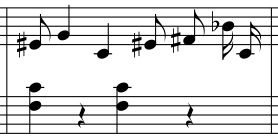
\includegraphics[scale=0.6]{figure/randomgenerationdifferentdurations.png}
  \captionof{figure}{Probabilistic generation with varying durations}
  \label{fig:probabilisticgenerationwithdifferentdurations}
\end{figure}

\subsection{Summary Of Non-Grammatical Approach}
The idea behind doing an initial non-grammatical probabilistic example is to show that first of all, rhythm is important in music. Different combinations of durations give us different rhythmic qualities, some of which sound wrong/awkward and some which sound pleasing. If we don't constrain the rhythmic aspects of the generated music then we end up with music that sounds random and unpleasing to the listener.
The other reason for doing the non-grammatical approach is that we can compare it to the results of using a grammar to generate music, thus allowing us to show the difference that using a grammar makes to the rhythmic aspects of the music.

\pagebreak

\chapter{Grammatical Approach}

\section{Introduction}
In this project we propose a grammatical approach for generating blues melodies. Grammars have been used in other works in the field of computer music improvisation (see Chapter 1 - Related Works). We hope to be able to compare our approaches and results to mathematical and machine learning techniques for music improvisation/generation. 'Finding temporal structure in music: Blues improvisation with LSTM recurrent networks' By Eck and Schmidhuber (2002) \cite{eck02} is a more recent example of using LSTM networks to generate jazz bebop melodies. However there is a need for a training set and the result is affected by the quality of the training set. Using a grammar means that we don't need to encode a training set or input set and can directly influence our resulting sound.

\section{Grammars and Music}
Grammars enforce structures within music and such a linguistic approach seems suitable for the 'call and response' nature of African-American influenced music such as blues \& jazz. We can compare a line of melody to a sentence in natural language. For example a sequence of notes and the rhythm that they occur in gives a melody it's own character and meaning, like a sentence in natural language. However in music there are no semantic rules in terms of the melody, it is entirely up to the listener/player as to how they interpret it. This is where a grammar comes in, grammars are structural rules that govern the composition of 'sentences' (in the case of natural language) and such grammars are not concerned with the semantics of the sentence. Therefore a well-defined grammar for blues music should be able to produce well-structured blues melodies.

\subsection{Issues With Grammars For Music} \label{grammarissues}
We acknowledge that there are some limitations for using grammars to generate music. A grammar has a finite search space and thus does not allow evolution of the improvisations of the program. Approaches that use inputs for training and analysing also suffer from the same problem too. However on the other hand we can come up with any grammar to use in the system which will in turn generate different pieces of music, much like other solutions that use machine learning / analytical approaches can generate different styles of music based on the given input training data.

\section{Adding a Grammar For Jazz}
The initial approaches are promising and give us a good foundation to build upon. If we randomly choose notes from a blues scale, they generally sound acceptable/good in terms of the pitch. However we have identified that some of the melodies/bars do not sound good rhythmically, i.e. they either don't sound good at all, or don't have the blues characteristics. We can see now that the rhythm of the notes is just as important as the pitch of the notes. 

In Keller and Madison's paper \cite{keller07}, a comprehensive grammar for blues is specified with excellent results. In particular a stochastic context-free grammar is used, where production rules of a context-free grammar are augmented with a probability/weighting. By using ideas from this approach we hope that we can create a more comprehensive grammar with more scope for variations. The terminal alphabet for the grammar is classified into different types of 'abstract tones'. A grammar can use these different types of tones to form a melodic sequence. The classification of different abstract tones is very much applicable to blues/jazz improvisation where knowledge of how to put these different types of tones together mean a better sounding melody is formed. In our previous non-grammatical examples, we use only notes from the blues scale. Though they sounded fine musically, using such a small set of notes means that the melody sounds flat and uninteresting for the most part and does not represent the widened Jazz musical genre. Additionally it is valid jazz to use notes that aren't part of the scale, they can be used as a 'passing note' for example and as such makes the melody sound more interesting and complete (see \ref{avoidnotes} on avoid notes). An article by Keller entitled 'How to Improvise Jazz Melodies' \cite{jazzkeller} talks about different methods for improvising blues/jazz melodies. The article provides many different methods and guidelines for improvising jazz/blues melodies. The above mentioned paper \cite{keller07} however only uses a few of these guidelines (albeit the most important ones). The classification of notes/tones are as follows:

\begin{description}
  \item[Chord Tones (\textit{C})] are tones (notes) which belong to the current chord we are improvising on top of.
  \item[Colour Tones (\textit{L})] are auxiliary tones for the current chord which sound correct musically when played with the current chord as an accompaniment. In particular, colour tones do not belong to the notes in the chord. 
  \item[Approach Tones (\textit{A})] are also notes which aren't in the chord (not the same as colour tones either) but they make good transitions to chord-tones or colour tones. These are also sometimes known as 'passing notes' where such a note can be placed between two chord/colours to make the melody seemed less disjointed. It is often bad practice however to place two approach tones next to each other.
  \item[Other] tones which don't belong to any of the above. These may include a rest \textbf{(\textit{R})}, or a scale tone \textbf{(\textit{S})} (a tone in the scale which works musically with the accompanying chord).
\end{description}

The issue we were concerned with before was whether we should deal with pitches of notes separately from the duration of the note. We have an option to create a grammar just for the rhythm of the melodic sequence. However randomly picking notes from the scale will not give us a result as good as the one in Keller and Madison 2007. The idea of chord, colour and approach tones provides us with a much better method of generating better sounding melodies.

\subsection{Context-Free Grammars}
The grammar described above is a context-free grammar. A grammar is considered context-free if the rules (production rules) of the grammar can be applied, i.e. the non-terminals can be written, without being dependant on the surrounding symbols. The majority of natural languages can be said to be based on context-free grammars. In addition we can say that the implementation of such a grammar for blues music is similar (and should be similar) to the implementation style of context-free grammars for random sentence generators. 

Context-free grammars are defined by the 4-tuple (V,$\Sigma$,R,S):

\begin{description}
  \item[V] - a finite set of \emph{variables}(non-terminal characters). Each variable essentially represents a different way to put together different families of notes and durations.
  \item[$\Sigma$]  - a finite set of \emph{terminals} which contain the actual content. In the case of our grammar, the terminals represent the type of tones/notes in the sequence.
  \item[R] - a set of production \emph{rules} in the form of A $\rightarrow$ b, where A is a variable $\in$V and b could be a sequence of variables and/or terminals.
  \item[S] - the starting variable/symbol used to represent the whole sentences where S$\in$V.
\end{description}


We start with starting variable S and expand the right hand side of the rule for S using other production rules. Expansion occurs by replacing variables in the sequence with the right hand side of the rule for that variable. We do this until the final result is a sequence of terminals only.

\subsubsection{Stochastic Context-Free Grammar}
The grammar that is defined in Keller's paper \cite{keller07} is a context-free grammar with probabilities, a stochastic/probabilistic context-free grammar. Each production rule has a probability associated with it which determines the likelihood of which production rule to use (if there are more than 1 with the same variable on the left hand side). The grammar specified below is such a grammar.

\section{Abstract Tone Grammar For Jazz}
We aim to implement the grammar described in the paper by Keller \cite{keller07} as a basis for jazz improvisations. The grammar itself is essentially a set of production rules which represent different rhythmic phrases with families of tones and their duration as the terminals. At the top level, we have the production rules P(n) $\rightarrow$ ... where n is the length of the melody generated in quarter/crotchet beats and n $\in$ 1..N:

\begin{verbatim}


P(0) -> empty [1]
P(1) -> Q1 [1] 
P(2) -> Q2 [1] 
P(3) -> Q2 Q1 [1] 
P(n) -> Q1 P(n−1)  [ .4 ]
P(n) -> Q2 P(n−2)  [ .4 ] 
P(n) -> Q4 P(n−4)  [ .2 ]

\end{verbatim}

A P variable takes in argument n, which limits the generation of the melody to fit n beats. We could also have a recursive grammar which expands until it reaches a set limit, but we may end up truncating a phrase which is not preferred. The values in the square brackets denote the weights for choosing a particular rule. It is worth noting that for the rules above, the weights are the same as probabilities (they add up to 1, so for P(n):  0.4+0.4+0.2 = 1), however it is not a requirement. The weights will will be normalised so that the actual probabilities are worked out.

The rest of the rules are taken from the aforementioned paper. We have rewritten the names of variables so that the numbers which follow a letter (i.e. Q4, V1, N/2 etc) denote the length of the notes generated (in quarter/crotchet beats). For example all the terminal sequences that can be generated from variable Q4 will have a total length of 4 crotchet beats. In addition, the number of beats that V/2 produces is half a beat (and also any other variable with /2). The specification of the grammar in Keller's paper \cite{keller07} is slightly inconsistent in the variable naming convention and can cause confusion. Therefore the rules (with new renamed variables) are as follows:

\begin{verbatim}

Q4 -> Q2 V1 V1  [0.52]
Q4 -> V/2 N1 N1 N1 V/2  [0.01]
Q4 -> V1 Q2 V1  [0.47]

Q2 -> N2  [0.06]
Q2 -> V1 V1  [0.6]
Q2 -> V/2 N1 V/2  [0.12]
Q2 -> H3/2 N/2  [0.16]
Q2 -> ({3} H1 H1 H1)  [0.06]

Q1 -> C1  [1]

V1 -> N1  [0.22]
V1 -> V/2 V/2  [0.72]
V1 -> ({3} H/2 H/2 H/2)  [0.05]
V1 -> ({3} H/2 H/2 A/2)  [0.01]

V/2 -> N/2  [0.99]
V/2 -> H/4 A/4  [0.01]

N2 -> C2  [1]

N1 -> C1  [0.5]
N1 -> L1  [0.2]
N1 -> S1  [0.5]
N1 -> A1  [0.01]
N1 -> R1  [0.25]
N/2 -> C/2  [0.4]
N/2 -> L/2  [0.2]
N/2 -> S/2  [0.4]
N/2 -> A/2  [0.01]
N/2 -> R/2  [0.1]

\end{verbatim}

In the N-variables, C, L, S, A and R are terminals in the terminal alphabet. They are shorthand for the families of tones that we've described at the beginning of the section. The grammar itself contains 4 distinct levels / types of variables:

\begin{description}
  \item[N-variables] - e.g. N2, N1 and N/2. These variables are at the bottom of the tree and their rule is always rewritten as a single terminal with the same length as the variable (see above).
  \item[V-variables]  - e.g. V1 and V/2. These are intermediate variables that describe small rhythmic sections. They allow the specification of different ways of making up a certain number of beats. For example we could add rules for V1 to represent more possible phrases, such as [V1 $\rightarrow$ H/4 N/2 H/4] if we wanted to add more variety to the music. They use the N-variables above to construct the sections. Note that the H-variable is a terminal which represents a \textbf{helpful} tone and refers to any of the Chord (\textit{C}), Colour (\textit{L}) and Approach (\textit{A}) tones.
  \item[Q-variables] - e.g. Q4, Q2, Q1. These are top level variables which essentially combine smaller sections/phrases to produce the larger sections. 
  \item[P-variable] - e.g P(n), the starting variable (as seen previously).
\end{description}

Again each rule has a probability associated with it and the above probabilities are taken from the above mentioned paper. The probabilities themselves play a large role in how the resulting melody sounds and at the moment can only be adjusted by the user.

Each unique derivation for each duration we generate for (the n in the P(n) starting variable) has its own unique parse tree. Figure \ref{fig:Q2parsetree} shows a partial parse tree just for Q2, which is already fairly comprehensive. We can see that the overall probability for generating a terminal sequence \emph{C1 C1} or \emph{C1 S1} from Q2 is 0.6x0.22*0.22*0.34*0.34= 0.00336. It is worth noting that many more melodies can be created with one particular terminal sequence, which we will discuss below.

The implementation of the above grammar will give the same results as in Keller's paper \cite{keller07}, indeed changes and enhancements may be made along the way to try and improve the result. 
It would also be better if we could allow users to adjust the grammar themselves to produce different melodies, for example a more complex grammar would perhaps produce a more complex melody. 

\begin{figure}[here]
  \centering
  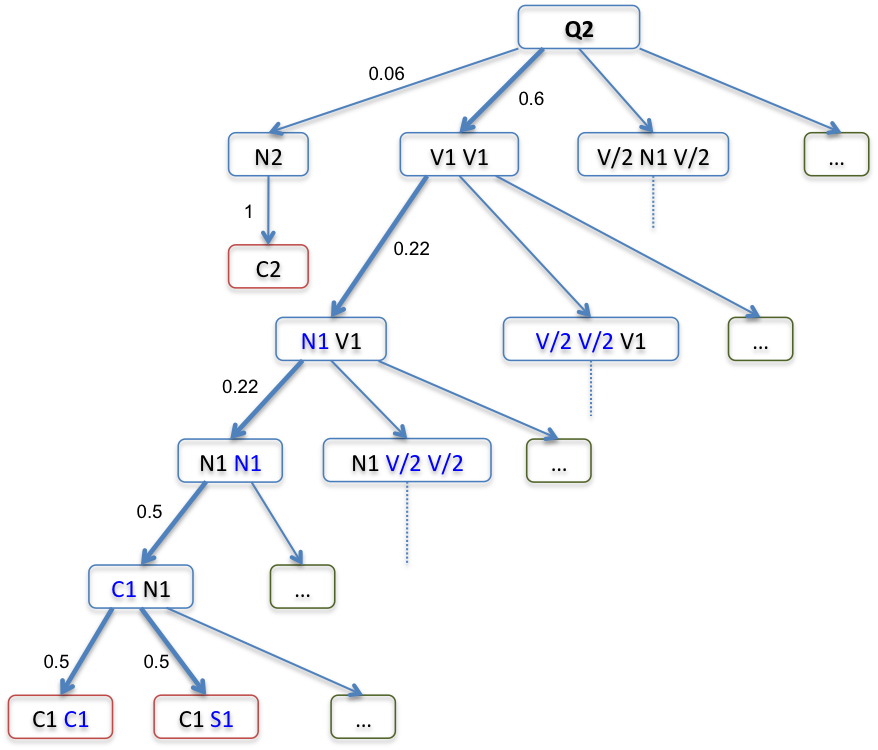
\includegraphics[scale=0.8]{figure/Q2parsetree.png}
  \captionof{figure}{Parse tree for Q2}
  \label{fig:Q2parsetree}
\end{figure}

\section{Terminal Sequences to Melodic Sequences} \label{terminalsequences}
As we've discussed previously, the grammar above generates a terminal sequence of types of tones and durations. Additional work needs to be done in order to produce a sequence of actual musical notes. An example terminal sequence that may be generated for P(4) $\rightarrow$ Q2 Q2 may be:

\begin{verbatim}
C/2 L1 H/4 A/4 H3/2 S/2
\end{verbatim}

We could generate many melodic sequences from the terminal sequence alone. However we would prefer to generate better sound melodies if possible. To do this we would have to introduce constraints when choosing actual musical notes from the families of tones, otherwise we may end up with a melody that sounds as random as our non-grammatical attempts. To do this we refer to Keller's article 'How to Improvise Jazz Melodies' \cite{jazzkeller}. Here are some possible ways we can constrain the selection of notes to ensure a better sounding melody:

\begin{description}
  \item[Know scales that go off the chords] scale here refers to a set of notes, rather than a sequence. If we know what scale works for the current chord, then it can help constrain the choice of tones so that the melody is closer to the scale.
  \item[Intervals between notes] smaller intervals often sound more pleasing than large intervals, however it is good to have both. If our intervals are too big then the melody will sound quite discordant (i.e. it will sound quite jumpy and erratic). However alternatively 'skipping' notes can sound good if combined with a direction change (see below) and can give a zig-zagged effect.
  \item[Change direction] if we have a sequence of small intervals (scale-like sequence) we may want to change direction at some point to provide variety and make the melody sound more interesting. We don't want to do this too often however as it may sound disorientating.
  \item[Use of enclosures] similar to direction changes, we can approach a note from both sides alternatively. This involves making sure intervals get smaller and also direction changes occur. Enclosures work better if the target tone is a chord tone.
\end{description}

By implementing these musical features, we can avoid awkward note combinations and optimise the melodic sequence from the terminal sequence.


\section{Heuristics \& Methods For Note Selection}
There are different ways we could select the final note sequence from the abstract tone sequence. However we are not trying to find the 'optimal' solution as in reality there is no optimal solution when it comes to music. We can only hope that by following some guidelines and rules (from \ref{terminalsequences}) we may be able to generate better sounding melodies. We also have to be careful to make sure that our rules are not too fine grained so that it limits the variety of what we can generate. Variety is important for music and it allows for a range of musical expression.

Jazz improvisation is similar to any other creative activity, in that experience accounts for much of the performance. We explore whether it is possible to encapsulate such experiences as heuristics to generate the final jazz melodies. The idea of using a heuristic is that we can capture the current knowledge and experience associated with basic musical composition (and note selection) and use that to generate the actual musical notes. 

\subsection{Initial Steps}
Previously we mentioned that two approach tones next to each other may not sound good (due to a high chance of there being dissonance). So the first step is to make sure that if we have an Approach tone followed by another Approach tone, we need to convert the second Approach Tone into a different tone (default is Chord tone).
The abstract grammar essentially restricts our note selections by giving us a terminal sentence consisting of abstract tones. The tones tell us which notes will work at this point in the sequence/phrase. Of course there is still a lot that we could do to determine which notes are picked and as we've mentioned previously, many melodic sequences could be generated from the terminal sequence. 

\subsection{Globals}
We intend to have some global limits for note selection for which all algorithms can use. This will be set as a properties file which can be read into the program. Currently we have an interval limit, which says how many semitones apart should the next note be within. In addition we also don't want to constrain the interval limit too much, sometimes having a large jump (octave changes for example) creates interest and variation, so we also set a probability that we select a note which has an interval from the previous note which is bigger than the interval limit. Finally we also set a maximum interval limit, such that no intervals between two notes can be bigger than this number. An example of what our properties file would look like is here:

\begin{verbatim}
intervalLimit = 5
intervalLimitProb = 0.95
maxIntervalLimit = 9
\end{verbatim}

\subsection{Simple Heuristic}
We initially came up with a simple heuristic in which the next note depends on the note that immediately precedes it. This simple approach of course does not take in account for many of the things we discussed in \ref{terminalsequences}. Most importantly, approach tones are not really approach tones as they are only dependant on the note before it, when they should be dependant on the note after it.
The algorithm is quite simple:

\begin{verbatim}

function convertTonesToNotes(listOfTones)
  listOfFinalNotes = []
  previousNote = null
  for tone in listOfTones:
    listOfNotes = getAvailableNotes(tone)
    if previousNote != null then
      listOfPotentialNotes = []
      for each note in listOfNotes then
        rand = random number
        if rand > intervalLimitProb then
          if interval(note, previous note) <= maxIntervalLimit then
            add note to listOfPotentialNotes
          else
            nothing
        else
          if interval(note, previous note) <= intervalLimit then
            add note to listOfPotentialNotes
      add random note from listOfPotentialNotes to listOfFinalNotes
    else
      add random note from listOfNotes to listOfFinalNotes
  return listOfFinalNotes

\end{verbatim}

The idea behind it is simple, we take each tone from the list of abstract tones (starting from the beginning) and we get a list of suitable notes that can use. Initially we can random choose from this list. For the next tone we again get the list of suitable notes that we can use and again randomly pick one note as long as it satisfies the global interval constraints.


\chapter{Reward-Based Learning Extension}

\section{Overview}
The problem with a grammar as we've discussed in \ref{grammarissues} is a finite search space, this may be more noticeable with a smaller grammar. Even though with a larger grammar we may not notice the generative limits of the grammar, the static aspect of the system does not represent improvisation by a human. Learning in humans is of course a complex process. But it is important to know that a human musician learns and continually improves over time, for example they may discover a new style to play music or find a new phrase/jazz lick which they enjoy the sound of. In order to make the program exhibit more human-like qualities we have come up with a reward based system which updates individual production rule weightings in the abstract tone grammar (see Chapter 4). The reward based system uses the user/listener as a fitness function (evaluation) in order to determine which grammar rule weightings to update. It can be said that this reward system that we use here is an abstraction and simplification of reinforcement learning, the states are the parse trees, actions are a collective process of choosing the rules to expand in the grammar for one parse tree and the reward is the user evaluation as the fitness function. The differences are that in this problem, we are not expecting to find a 'maximum expected return' as music has no real optimal result and the process of choosing an action to take is stochastic.

\section{Approach}
As the user is listening to sequences of notes, their response/feedback is based on both the rhythmic qualities of the note and the pitch of the notes themselves (the pitch changes in reality), however in this approach we are only going to update our abstract tone grammar. The grammar is responsible for the rhythmic aspect of the music, however it also plays a role in determining and narrowing down the resulting notes that can be used. In essence, we need to be able to determine from the evaluation whether the listener selected the bar based on the pitch changes or the based on the grammar rules (mainly the rhythmic aspect). 

To do this we ideally do not want to iteratively update our grammar. A batch method would allow us to infer after many instances of feedback whether a particular grammar rule generates more pleasing sounding music. As the process of evaluating a piece of music is not quick (i.e. a person has to listen to the whole piece, probably more than once to provide accurate feedback) we only show a small amount of examples to the user (around 5-10). This should prove enough as each piece of music produces many parse trees.

\section{Fitness/Evaluation Function}
The fitness function is essentially going to be the user/listener. It is difficult to define a fitness function computationally as music is a very subjective thing. Even if we were to define a fitness function from the viewpoint and tastes of one person, it is also extremely difficult to formally describe what makes one sequence of notes sound better than another sequence of notes. We can abstract this away by using a human as the evaluator / fitness function.

\section{Rule Update \& Example}

A simple example would be show the user a selection of melodic sequences. The listener would indicate which bars sound particularly pleasing. We can then identify which rules were used to generate such bars, i.e. identify the parse tree for a sentence. For example lets take the terminal sequence of abstract tones: [H/4, A/4, C1, S/2, C1, H/3, H/3, H/3]. The parse tree for the terminal sequence is shown in \ref{fig:q4exampleparsetree}.

\begin{figure}[here]
  \centering
  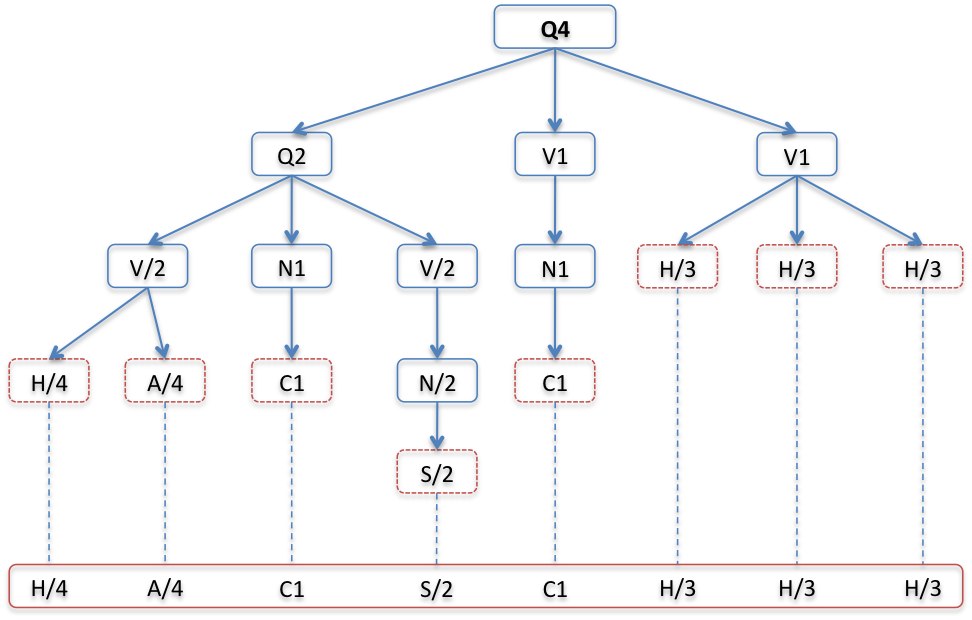
\includegraphics[scale=0.85]{figure/q4exampleparsetree.png}
  \captionof{figure}{Parse tree for the terminal sequence}
  \label{fig:q4exampleparsetree}
\end{figure}

Initially it would seem that if we were to adjust every rule then it would be mean our grammar weighting changes very easily. However if are increasing the weighting of a rule, we are essentially also decreasing the weighting of the the rules with the same variable. Adjusting many of the rules means we get a balanced weighting at the end. However this simple method is still not ideal as it would update/increasing the weighting of each rule by the same amount.

Ideally we'd want to be able to see after a batch run whether some rules have been selected more often than other rules. As a result we don't want to change all the rules, but only the ones that have been selected enough to strongly infer that they are responsible for generating the rhythmic aspect of the bars that were selected. In addition as our grammar is represented in a hierarchical tree structure, the leaves (N-rules) are likely to occur many times in a parse tree, compared to rules higher up the tree (Q or V rules). For example N1 $\rightarrow$ C1 is likely to come up more than once in a parse tree compared to a V rule, such as V1$\rightarrow$ H/3 H/3 H/3 (as seen in \ref{fig:q4exampleparsetree}). We also only get one Q4 and Q2 rule for each parse tree. 

A possible solution is to compare rules on the same level in the grammar hierarchy with each other. I.e. only compare N-rules against each other and 

Problem: can't just look at the number of times a rule was used, because some of the rules are designed to be the leaves in the parse tree, meaning that in a parse tree, those rules (N rules) will be used quite often compared to the higher level rules. So number of times occured does not really count. May need to see number of times occured relative to each seperate parse tree?


we need a way to determine which rules we would want to adjust the weightings of. We need to consider the number of examples that we've used and also the number of bars that were selected to be pleasing 


[[We can then perform crossovers of pairs of sequences to produce children. Crossovers could include swapping phrases around at the same place in the piece. We could then perform mutations on the child sequences such as altering the rhythm of a section. We would allow the fittest/best sounding sequences to be used more often for crossover, thereby producing better child sequences.

Crossover may also be done using terminal sequences (chord, colour approach tones etc) and not the actual sequence of notes. The reason for this is that swapping phrases of actual notes may result in disjointed sequences.]]

\chapter{Implementation}

\section{Overview}
The implementation of the blues improvisation using the grammar specified above will be primarily done in Java. Development will be done in the Eclipse IDE which provides good support including refactoring tools and auto-completion. Build management of the project is handled by Apache Maven, which manages dependencies and plugins required for the project. 

\section{Software Engineering Practices}
Software development is very much an iterative and incremental process. It is difficult to design the system correct on the first try and thus a lot of refactoring and changes may need to be done during the development process. In addition we hope that this piece of software forms a basis and platform upon which additional features can be implemented on top of. With both of these things in mind, it is important to make the system flexible and easy to extend. 

\subsection{Package Dependency/Management}
The program has been developed with software engineering considerations in mind. Classes are placed into appropriate packages such that packages do not have circular dependencies. [Show package dependency diagram?]. Interfaces are used to invert dependencies between packages and therefore reduce coupling in the system. 

\subsection{Extendability}
One of the aims of this project is that by making the program extendable, someone else can use the program as a foundation or basis for either exploring/implementing additional features or extending current features (such as a more comprehensive chord-scale system). As we shall see in the next section, by separating out the code to represent musical objects (things in the musical domain) we have offered a library that other users can use to represent and manipulate music with.

\section{Representation of Musical Objects}

\subsection{ABCJavaMusic}
In order to make manipulating musical notes easier, we decided to write a separate library (ABCJavaMusic) which allows us to represent musical notes/objects as java objects and represent/output them as ABC notation (see section 3.1). We could have used existing libraries and tools to convert from our abstract grammar to a musical score such as abc4j\footnote{http://code.google.com/p/abc4j/}. abc4j provides a parser that parses abc music files and in addition many features such as midi playback and music score display. Whilst these are useful things, other external tools can be used to achieve this often with better results, such as Ernie\footnote{http://geophysics.kos.net/ernie/} on Mac OSX (which can do midi playback and musical score display).

However the thing we are concerned with is the musical model. The musical model allows us to manipulate notes which is important as our computer essentially acts as the creative brain for generating notes. abc4j's musical model is very verbose and very similar to how abc notation itself represents music. 
ABCJavaMusic on the other hand represents music using a hierarchical structure as follows:

\begin{verbatim}
Full Score Line
  ->Treble/Bass Clef Score Line
    ->Bar
      ->Phrase
        ->Timed - Note Component (with duration)
          ->Note Component (with octave and accidental)
            ->Basic Note (with accidental)
\end{verbatim}

Having a hierarchical structure is useful as sometimes we may want information about a phrase, or about an individual note component. It is therefore beneficial overall to create a small/light-weight set of classes which do exactly what we want. This way, users can use this library to manipulate the musical objects for purposes similar to this project. Currently the objects can only print out as ABC notation.

\subsubsection{Example}
Here we demonstrate how we would represent some simple notes as Java objects. In Figure \ref{fig:abcnotationexample}, if we want to represent the notes as ABC notation (disregarding headers and bar lines in the ABC file) then it would look like:

\begin{verbatim}
C _D ^F3/2 _B,/2
\end{verbatim}

Where '$\_$' represents a flat, '$\wedge$' represents a sharp, and the ',' represents a lower octave (an apostrophe ['] represents a higher octave). The duration of the note (in this case in quarter/crotchet beats) is the number directly after the pitch of the note (C, D, E all have a duration of 1 quarter beat). So F\# and B both have /2 which indicates the duration is half of a quarter/crotchet beat, i.e. an eighth/quaver.

In Java, we would represent these notes by writing this code:

\begin{lstlisting}
MainNoteComponent middleCNote = 
      new MainNoteComponent(BasicNote.C);
TimedComponent middleCNoteQuarter = 
      new TimedComponent(middleCNote, Duration.quarter);

MainNoteComponent DFlatNote = 
      new MainNoteComponent(BasicNote.D, AccidentalShift.Flat);
TimedComponent DFlatNoteQuarter = 
      new TimedComponent(DFlatAboveMiddleCNote, Duration.quarter);

MainNoteComponent FSharpNote = 
      new MainNoteComponent(BasicNote.F, AccidentalShift.Sharp);
TimedComponent FSharpNoteDottedQuarter = 
      new TimedComponent(FSharpNote, Duration.dottedQuarter);

MainNoteComponent BFlatBelowMiddleCNote = 
      new MainNoteComponent(BasicNote.B, AccidentalShift.Flat, -1);
TimedComponent BFlatBelowMiddleCNoteEighth = 
      new TimedComponent(BFlatBelowMiddleCNote, Duration.eighth);

\end{lstlisting}

To represent a bar with those notes (all in one phrase), we would write:

\begin{lstlisting}
Bar bar = new Bar();
StandardTimedComponentPhrase phrase = 
      new StandardTimedComponentPhrase();
phrase.addtoComponentList(middleCNoteQuarter);
phrase.addtoComponentList(DFlatNoteQuarter);
phrase.addtoComponentList(FSharpNoteDottedQuarter);
phrase.addtoComponentList(BFlatBelowMiddleCNoteEighth);
bar.addToBar(phrase);

\end{lstlisting}

By calling bar.getAbcRepresentation() we would get the abc representation of these notes as seen above. The representation is very verbose, however it is not intended to be used to represent complete pieces of music. ABC notation is designed for the actual music representation. For example in our system, we use the library to convert the terminal sequence from our grammar (sequences of Tones) to actual musical notes, using heuristics / probabilistic methods. 

In addition if we wanted to get a full score line then we could do the following:

\begin{lstlisting}
TrebleClefScoreLine trebleClefScore = new TrebleClefScoreLine();
trebleClefScore.addBarToScoreLine(bar);
//we don't have anything in the bass clef, 
//so we just use a default empty bass clef score line
CombinedScoreLine fullScore = 
	new CombinedScoreLine(trebleClefScore, 
			      BassClefScoreLine.emptyScore());

\end{lstlisting}

\begin{figure}[here]
  \centering
  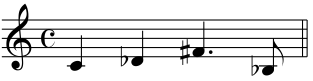
\includegraphics[scale=0.6]{figure/abcnotationexample.png}
  \captionof{figure}{Notes C, Dflat, Fsharp and Bflat}
  \label{fig:abcnotationexample}
\end{figure}

\subsection{ABC Notation}
ABC notation is a text-based music notation system which allows simple representation of musical scores. It is widely used in folk and traditional music and is ASCII based. There is support for the format including tools to convert abc notation to midi and to printable scores (as pdf's). More about the notation can be read on the website \url{abcnotation.com}.

\section{Grammar Implementation}
Numerous options have been explored for implementing the grammar (along with generation of sequences) in Chapter 2, section 3.2. The main options are:

\begin{description}
  \item[Parser Generator Tools] such as ANTLR, which allows a context-free grammar to be specified using Extended Backus Naur Form and can generate lexers and parsers. It's main use is for generating a recogniser for a language define by the context-free grammar which checks the syntax of the input (a sample program in the specified language). ANTLR also has a maven plugin which can manage compilation of grammars.
  \item[External Languages] such as Python, or Lisp. These dynamic languages are useful for specifying a context-free grammar and generating sentences/sequences from the grammar. In particular in Lisp, a grammar can conveniently be expressed using s-expressions, a notation to represent a nested list hierarchy. Similarly a grammar can be represented using dictionaries in Python. Python has parsing libraries which can be used to create a parser and lexer for the inputted grammar file.
  \item[Native Implementation in Java] would keep the codebase all in one language. The implementation of the grammar may not be as straightforward as in Python or Lisp as we would have to represent everything as objects in Java. This approach is feasible if the grammar is small. However if we were to expand the grammar in the future then this may not be the best option.
\end{description}

We decided in the end to use Python parse the input grammar and to do sequence generation. Python is currently preferred due to existing experience and also the functional aspects of Python are ideal for sentence generation from a tree. As we want to be able to use both Java and Python together, we can use Jython, an implementation of Python written in Java (i.e. it runs on the JVM). This way we can invoke Python code from Java, allowing us to store our specified grammar in Python and invoke Python methods to generate sequences from the grammar. 
In terms of parsing the grammar, we used the PyParsing library, which allow us to represent the grammar to parse the musical grammar. 

\chapter{Evaluation}

\section{Overview}
We hope that the project can contribute something towards the field of creative music improvisation. By building on existing grammatical approaches and by incorporating rules and techniques that we as humans learn when start learning how to play/improvise, we aim to be able to improve the standard of generated music so that it resembles human-played music. Additionally, we hope that such a tool can help and aid people who want to learn blues improvisation by generating simple melodies and phrases for them to practise with.  

\section{Measuring Success}
As we are improving on existing work laid out in Keller's paper \cite{keller07}, we could say that we can judge the success of the project by judging whether the new generated blues music sounds 'better' than the music generated by just the grammar alone in Keller's paper.

However it is not easy by any means to judge whether one piece of music is 'better' than the other piece of music. Of course we could say that being more pleasing to the ears is main criteria, but the auditory experience of a piece of music is subjective from person to person. We could use other criteria to judge the success of our efforts, for example we could say that the complexity of phrases and whether it matches up to phrases/licks in blues music composed by humans could form the basis of our assessment.

We would also want to compare whether our grammatical approach produces better results than a machine learning approach. It is also important to consider the scope of the music that we can generate using a grammar compared to using machine learning. For example machine learning techniques mean that a program can continually learn and train to produce better sounding / more complex pieces, whereas a grammar is constrained and limited in it's search space. 



\bibliographystyle{plain}
\bibliography{refs}

\end{document}


